% Complete Section 7.6, original PDF 100-101 / printed 90-91.
% block: whitney-forms-de-rham-heading page:100 type:section
\subsection{{The Whitney forms $\mathcal P_1^-\Lambda^k$ and de Rham's theorem}}\label{sec:whitney-forms-de-rham}

% block: whitney-forms-geometric-dofs page:100 type:ordinary-paragraph
{The lowest degree trimmed polynomial finite element space $\mathcal P_1^-\Lambda^k(\mathcal T_h)$ is a subspace of $H\Lambda^k(\Omega)$. Its elements are called the \emph{Whitney $k$-forms}. Its shape functions $\mathcal P_1^-\Lambda^k=\mathcal P_0\Lambda^k+\kappa\mathcal P_0\Lambda^{k+1}$ form a subspace of the complete space $\mathcal P_1\Lambda^k$ of linear polynomial $k$-forms (a proper subspace if $k>0$). Figure~\ref{fig:whitney-form-dofs} shows element diagrams representing the four spaces $\mathcal P_1^-\Lambda^k$, $0\leq k\leq3$, in three dimensions. Each element diagram shows a single simplex with a symbol placed on a face to mark each DOF occuring there. Notice that the DOFs of the Whitney forms are highly geometric: for the Whitney $k$-forms, there is precisely one DOF on each $k$-dimensional subsimplex---namely, the integral of the trace over the faces---and none on the faces of other dimensions. In fact, these spaces appeared in the book \BookCite{70} of Hassler Whitney in 1957, independently of finite elements.}

% block: whitney-form-complex pages:100,101 type:ordinary-paragraph
{As we have seen, the Whitney forms assemble to form a cochain complex:}
\begin{equation}\label{eq:whitney-form-complex}
0\to\mathcal P_1^-\Lambda^0(\mathcal T_h)\xrightarrow{d}\mathcal P_1^-\Lambda^1(\mathcal T_h)\xrightarrow{d}\cdots\xrightarrow{d}\mathcal P_1^-\Lambda^1(\mathcal T_h)\to0,
\end{equation}
{which is a discrete subcomplex of the $L^2$ de Rham complex associated to the triangulation $\mathcal T_h$. We also recall that the Whitney forms in $\mathcal P_1^-\Lambda^k(\mathcal T_h)$ have well-defined traces on the $k$-faces. Indeed, that the traces on $k$-faces are single-valued is part of the definition of the space.}
\footnote{{In fact, the trace of a Whitney $k$-form on a $k$-face $f$ is a constant $k$-form, since it belongs to $\mathcal P_1^-\Lambda^k(f)$ and on a $k$-dimensional domain, $\mathcal P_1^-\Lambda^k$ reduces to $\mathcal P_0\Lambda^k$.}}
{Therefore, the de Rham map $F^k$, which takes differential $k$-forms to $k$-cochains, is well-defined on the Whitney forms:}
\[
F^k\phi(g)=\int_g\operatorname{tr}_g\phi,\qquad\phi\in\mathcal P_1^-\Lambda^k(\mathcal T_h),\quad g\in\Delta_k(\mathcal T_h).
\]

% block: whitney-form-dofs-figure page:101 type:figure
\begin{figure}[htbp]\centering
\includegraphics[page=101,trim=112bp 572bp 85bp 62bp,clip,width=.90\linewidth]{../input/source/Finite Element Exterior Calculus.pdf}
\caption{{DOFs for the Whitney forms in three dimensions.}}\label{fig:whitney-form-dofs}
\end{figure}

% block: whitney-simplicial-cochain-isomorphism page:101 type:ordinary-paragraph
{Notice that the values $F^k\phi(g)$ are just the DOFs of $\phi$: they can be assigned arbitrarily and uniquely determine an element of $\phi$. This is just another way to say that the de Rham map $F^k$ defines an isomorphism of space $\mathcal P_1^-\Lambda^k(\mathcal T_h)$ of Whitney $k$-forms onto the space $C^k(\mathcal T_h)$ of simplicial $k$-cochains. The collection of these isomorphisms, as we vary $k$, form a cochain map, as we already saw in Chapter~\ref{chap:homological-algebra}. In short, \emph{the de Rham map is a cochain isomorphism between the Whitney form complex and the simplicial cochain complex}.}

% block: whitney-proof-of-de-rham-theorem page:101 type:ordinary-paragraph
{We can use the Whitney forms to prove a version of de Rham's theorem, which we stated at the end of Chapter~\ref{chap:homological-algebra}. The cohomology associated to the Whitney form complex \eqref{eq:whitney-form-complex} is certainly isomorphic to the simplicial cohomology. Indeed, the complexes themselves, not just their cohomology, are isomorphic. But now consider a bounded cochain projection, which we know exists, from the $L^2$ de Rham complex to the Whitney complex. By Theorem~\ref{thm:discrete-cohomology-isomorphism}, this induces an isomorphism of the de Rham cohomology onto the cohomology of the Whitney complex, as long as the approximation property \eqref{eq:harmonic-projection-strict-error} holds. This is certainly true if the mesh size is sufficiently small, which can always be obtained by refining the mesh. But it is in fact true for any mesh, since the simplicial cohomology is easily shown to be unchanged by refinement.}

% block: de-rham-cohomology-isomorphism-qualification page:101 type:remark
\Needspace{8\baselineskip}
\begin{Remark}\label{rem:de-rham-cohomology-isomorphism}
{We have proven that the $L^2$ de Rham cohomology is isomorphic to the simplicial cohomology. De Rham's theorem is more typically stated in terms of the smooth de Rham cohomology, but this is not a significant difference, since the smooth and $L^2$ de Rham cohomology are themselves isomorphic via the inclusion map, essentially due to elliptic regularity. See [\BookNumber{24}, Theorem 2.12]. More significant is that the isomorphism we have given is induced by the smoothed projection operators (bounded cochain projections), rather than by the de Rham map, which is not defined on the full $H\Lambda^k$ spaces.}
\end{Remark}
